\chapter{SUBESTAÇÕES DE ENERGIA ELÉTRICA}

Todo sistema de potência é constituído de três diferentes segmentos: geração, transmissão e distribuição \cite{mamede2011subestacoes}. Para que a energia gerada no primeiro segmento chegue ao seu destino final, que é o consumidor que está ligado no sistema de distribuição, é necessário também que exista em cada um desses segmentos uma subestação que possa elevar e reduzir a tensão em diferentes níveis \cite{mamede2011subestacoes}.

Segundo Barros et al. \citeyearpar{barros2009cabine} a subestação primária compreende instalações elétricas e civis, e é destinada a alojar medição, proteção e transformação. Formada por um conjunto de equipamentos que devem atender às necessidades de fornecimento de energia elétrica das instalações por ela alimentadas, permitindo sempre a flexibilidade de manobras, a acessibilidade para manutenções, a confiabilidade quanto à proteção e à operação, e a segurança tanto para os equipamentos quanto para o pessoal envolvido.

Segundo Frontin \citeyearpar{frontin2013equipamentos}, uma subestação se desenvolve em várias etapas [...], com base em estudos específicos é definida a configuração de barra da futura subestação. Também são definidas as principais características dos equipamentos elétricos do pátio de manobras, bem como as características do sistema de proteção e controle. 

%%======================================================================

\section{Tipos de Elementos}

%%======================================================================

\section{Tipos de Barramentos}

As subestações são dotadas de barramentos nos quais são conectados tanto os circuitos alimentadores como os circuitos de distribuição, incluindo os transformadores de potência \cite{mamede2000protecao}. Existem vários tipos de arranjo de barramentos primários e secundários, que [...] deverá ser selecionado em função das características da carga, dos níveis de confiabilidade e continuidade desejados, do nível de flexibilidade de manobra e recomposição da subestação \cite{mamede2000protecao}.

\subsection{Barramento Simples}

O arranjo do barramento simples no primário é o mais básico e econômico de uma subestação. Sendo utilizado para munir subestações com tensão de até 69 kV, de pequeno porte. Sua confiabilidade é baixa, comparado aos demais, devido à perdas dos circuitos, quando ocorre incidentes na subtransmissão (Ver Figura \ref{fig:BarraSimplesPrimario}).

\begin{figure}[!htb] 
    \centering
    \caption{Proteção Barramento Simples}
    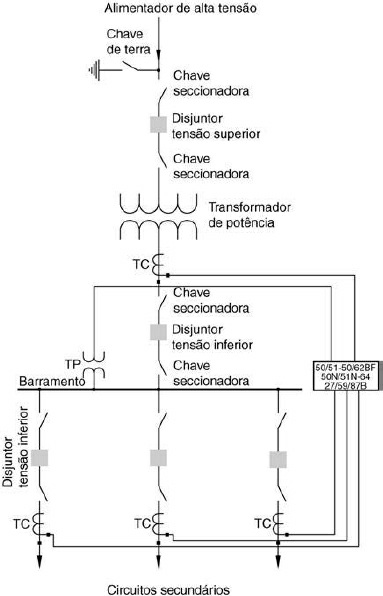
\includegraphics[scale = 0.9]{figuras/BarraSimplesPrimario.png}
    \\ Fonte: \cite{mamede2000protecao}
    \label{fig:BarraSimplesPrimario}
\end{figure}


\subsection{Barramento Simples com Barra de Transferência}

O barramento simples com barra de transferência, apresentado na figura \ref{fig:BarraTransferencia}, é utilizada em subestações de média e alta tensão. As manobras são realizadas sem que haja desligamentos e somente pode ser liberado um disjuntor de cada vez \cite{frontin2013equipamentos}. Esta configuração apresenta certa flexibilidade para manutenção e reparos, mas sua flexibilidade operativa é limitada, pois opera somente um barramento que limita a sua disponibilidade para ocorrência de falhas na barra e seccionadoras \cite{azevedo2015arranjos}. 

\begin{figure}[!htb] 
    \centering
    \caption{Proteção Barramento Simples com Barra de Transferência}
    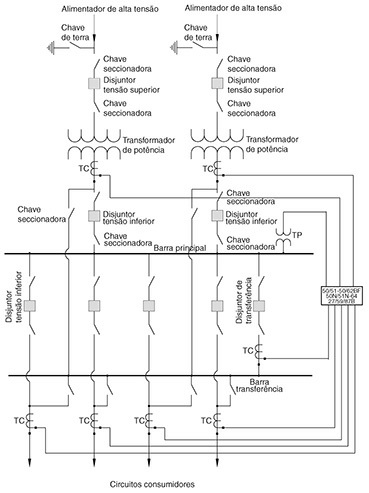
\includegraphics[scale = 1]{figuras/BarraTransferencia.png}
    \\ Fonte: \cite{mamede2000protecao}
    \label{fig:BarraTransferencia}
\end{figure}


\subsection{Barramento Simples Com Seccionamento de Barra}

O barramento simples com seccionamento de barra, apresentado na figura \ref{fig:BarraSeccionada}, é indicado para a condição de alimentação da subestação de dois ou mais circuitos de alta tensão e/ou quando há necessidade de se utilizar uma grande quantidade de circuitos de distribuição \cite{mamede2000protecao}. A flexibilidade para a manutenção das secções de barras tem uma sensível melhora, mantendo-se a subestação parcialmente em operação \cite{frontin2013equipamentos}.

\begin{figure}[!htb] 
    \centering
    \caption{Proteção Barramento Simples Com Seccionamento de Barra}
    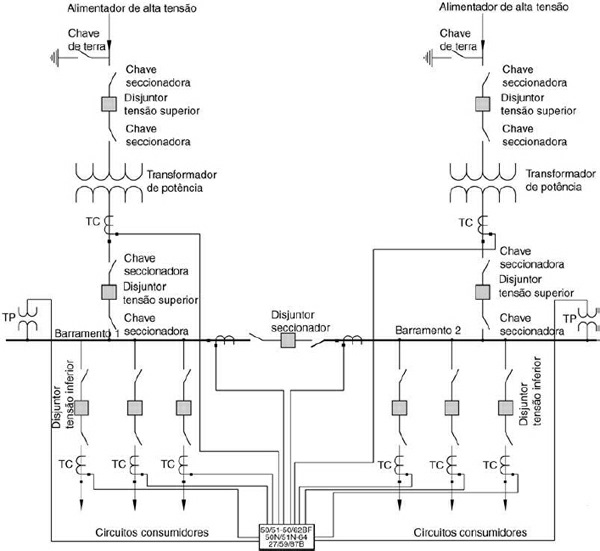
\includegraphics[scale = 0.7]{figuras/BarraSeccionada.png}
    \\ Fonte: \cite{mamede2000protecao}
    \label{fig:BarraSeccionada}
\end{figure}


\newpage

\subsection{Barramento Simples com Geração Auxiliar}

O barramento simples com geração auxiliar é semelhante ao arranjo anterior, com a diferença da fonte de geração auxiliar estar conectada à um dos barramentos (Ver Figura \ref{fig:BarraComGeracaoAuxiliar}). É indicado quando se necessita operar uma usina de geração termelétrica para funcionamento em emergência, na ponta de carga ou no controle da demanda por injeção de geração \cite{mamede2000protecao}.

\begin{figure}[!htb] 
    \centering
    \caption{Proteção Barramento Simples Com Geração Auxiliar}
    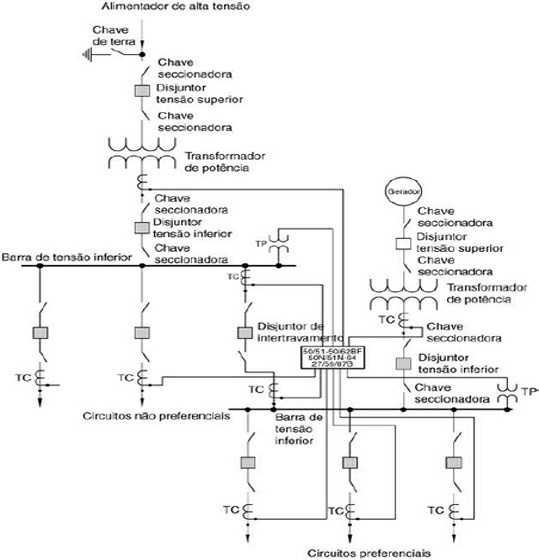
\includegraphics[scale = .75]{figuras/BarraComGeracaoAuxiliar.png}
    \\ Fonte: \cite{mamede2000protecao}
    \label{fig:BarraComGeracaoAuxiliar}
\end{figure}


\newpage

\subsection{Barramento Duplo a Quatro Chaves}

O barramento duplo a quatro chaves, apresentado na figura \ref{fig:BarraDupla4Chaves}, possui boa flexibilidade operativa e facilidades para a expansão, uma vez que se pode liberar temporariamente uma barra e não provocar desligamentos de circuitos do sistema \cite{holanda2016suel}. Nesta configuração, acrescenta-se uma chave de \textit{bypass} em cada \textit{bay}, de forma que todo disjuntor possa ser liberado para manutenção e reparos sem que seja necessário desligar o circuito correspondente \cite{frontin2013equipamentos}.

\begin{figure}[!htb] 
    \centering
    \caption{Proteção Barramento Duplo a Quatro Chaves}
    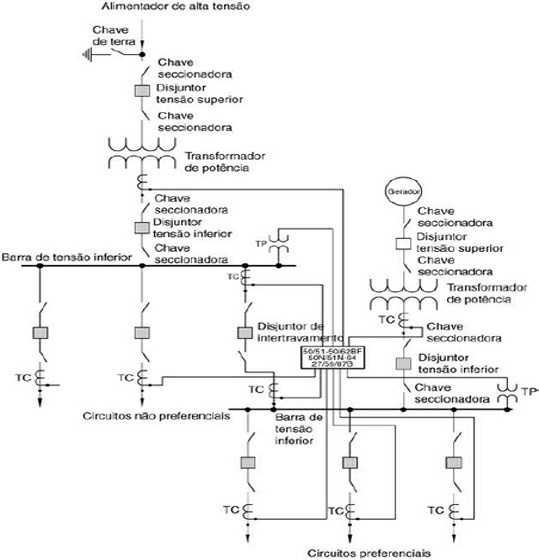
\includegraphics[scale = .8]{figuras/BarraComGeracaoAuxiliar.png}
    \\ Fonte: \cite{mamede2000protecao}
    \label{fig:BarraDupla4Chaves}
\end{figure}


\newpage

\subsection{Barramento Disjuntor Duplo}

O barramento disjuntor duplo, apresentado na figura \ref{fig:BarraDijuntorDuplo}, é caracterizado pela conexão dos circuitos de distribuição no ponto central entre
os dois barramentos \cite{mamede2000protecao}. Neste barramento a carga associada não é interrompida, caso ocorra um defeito em qualquer disjuntor dos circuitos secundários. 

\begin{figure}[!htb] 
    \centering
    \caption{Proteção Barramento Disjuntor Duplo}
    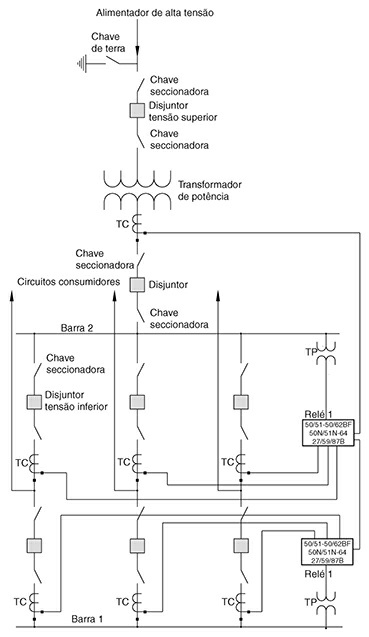
\includegraphics[scale = .8]{figuras/BarraDijuntorDuplo.png}
    \\ Fonte: \cite{mamede2000protecao}
    \label{fig:BarraDijuntorDuplo}
\end{figure}


\newpage

\subsection{Barramento Duplo e Disjuntor e Meio}

No barramento duplo e disjuntor e meio, apresentado na figura \ref{fig:BarraDijuntorMeio}, cada circuito pode ser alimentado por qualquer um dos barramentos por meio de um disjuntor central, que pode ser compartilhado por dois circuitos \cite{mamede2000protecao}.

\begin{figure}[!htb] 
    \centering
    \caption{Proteção Barramento Duplo e Disjuntor e Meio}
    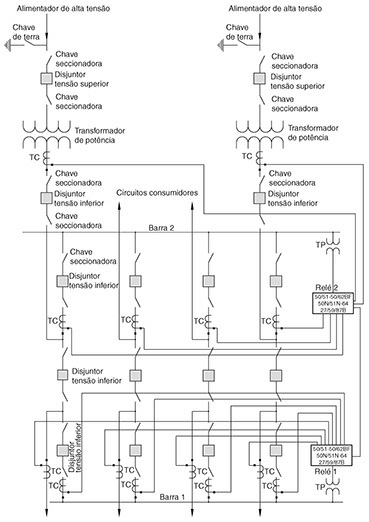
\includegraphics[scale = 1]{figuras/BarraDijuntorMeio.png}
    \\ Fonte: \cite{mamede2000protecao}
    \label{fig:BarraDijuntorMeio}
\end{figure}


\newpage

\subsection{Barramento em Anel}

Nesta configuração de barramento anel, embora econômica e flexível, tem o inconveniente de expor o sistema elétrico devido a falhas externas ao pátio em segundas contingências \cite{frontin2013equipamentos}. Segundo Holanda \citeyearpar{holanda2016suel}, apresenta a vantagem de dividir as cargas e controle do nível de falhas. Por outro lado, requer maior área de pátio em relação ao esquema de barra simples equivalente e quando um disjuntor estiver em manutenção, a abertura do outro
disjuntor não adjacente irá dividir o anel, podendo causar sérias perturbações no sistema.


\begin{figure}[H] 
    \centering
    \caption{Proteção Barramento Anel}
    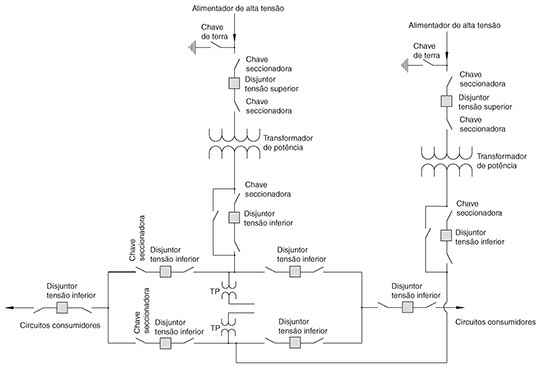
\includegraphics[scale = 1]{figuras/BarraAnel.png}
    \\ Fonte: \cite{mamede2000protecao}
    \label{fig:BarraAnel}
\end{figure}

%%======================================================================

\section{Tipos de Manobras}
